\chapter{Tìm hiểu kiến trúc AI Engine trên chip Versal.}
\begin{quote}
    Thời gian nghiên cứu: tuần 1, tuần 2, tuần 3.
\end{quote}

\section{Giới thiệu về AI Engine và Versal}

Versal là dòng chip mới của AMD/Xilinx, thuộc nhóm ACAP (Adaptive Compute Acceleration Platform), kết hợp nhiều loại tài nguyên tính toán: CPU, FPGA, và đặc biệt là AI Engine (AIE). AI Engine là bộ xử lý vector hiệu năng cao, tối ưu cho các tác vụ xử lý tín hiệu số (DSP), học máy, và các phép toán ma trận.

Các điểm nổi bật của Versal và AI Engine:
\begin{itemize}
    \item \textbf{Versal ACAP}: Tích hợp CPU ARM, logic lập trình (FPGA), và AI Engine, cho phép xử lý linh hoạt, hiệu năng cao, phù hợp nhiều ứng dụng từ mạng, xử lý ảnh, đến AI.
    \item \textbf{AI Engine}: Là tập hợp các tile xử lý song song, mỗi tile gồm bộ xử lý SIMD VLIW, bộ nhớ riêng, DMA, và giao tiếp streaming. AIE giúp tăng tốc các thuật toán tính toán nặng như nhân ma trận, FFT, inference AI.
    \item \textbf{Kiến trúc linh hoạt}: Versal cho phép kết nối giữa các khối chức năng qua mạng NoC, hỗ trợ truyền dữ liệu tốc độ cao, cấu hình động, và tối ưu hóa tài nguyên cho từng ứng dụng.
\end{itemize}

Nhờ sự kết hợp này, Versal và AI Engine mở ra khả năng tăng tốc phần cứng cho các ứng dụng hiện đại, đồng thời vẫn giữ được tính linh hoạt của FPGA truyền thống.
\section{Versal Adaptive Compute Acceleration Platform (Versal ACAPs)}

Versal ACAPs có \textbf{3 loại Engine} chính:

\begin{enumerate}
    \item \textbf{Scalar Engines (CPU)}
    \begin{itemize}
        \item Là các lõi ARM:
        \begin{itemize}
            \item \texttt{Cortex-A72}: CPU hiệu năng cao, chạy Linux, xử lý phần mềm ứng dụng.
            \item \texttt{Cortex-R5F}: CPU thời gian thực, dùng cho các tác vụ điều khiển (real-time).
        \end{itemize}
        \item $\Rightarrow$ Dùng cho quản lý hệ thống, khởi động, điều phối AI Engine, xử lý điều kiện...
    \end{itemize}

    \item \textbf{Adaptable Engines (PL - Programmable Logic)}
    \begin{itemize}
        \item Tương tự như FPGA truyền thống: logic block, LUT, DSP, BRAM.
        \item Lập trình bằng Verilog/VHDL/HLS (High-Level Synthesis C++).
        \item $\Rightarrow$ Dùng khi cần tuỳ biến thuật toán hoặc xử lý dữ liệu đặc thù, không cố định.
    \end{itemize}

    \item \textbf{Intelligent Engines (AI Engines -- điểm nhấn của Versal)}
    \begin{itemize}
        \item Là \textbf{các tile AI Engine} chứa:
        \begin{itemize}
            \item SIMD VLIW processor: xử lý vector hiệu năng cao.
            \item Bộ nhớ nội bộ (32KB), DMA.
            \item Stream kết nối với tile khác.
        \end{itemize}
        \item Dùng để xử lý \textbf{tín hiệu (DSP), machine learning, nhân ma trận, nhận dạng, inference}\ldots
    \end{itemize}
\end{enumerate}
\section{AI Engine Array Features}

AI Engine Array bao gồm \texttt{AIE tiles} và \texttt{AIE array interface} (gồm Network on Chip và PL).

\paragraph{AIE Tiles:}
\begin{itemize}
    \item Mỗi tile là một khối riêng biệt, nằm ngoài PL.
    \item Bao gồm một bộ xử lý VLIW SIMD tối ưu cho xử lý tín hiệu và học máy.
    \item Có 8 bank RAM đơn cổng, tổng cộng \textbf{32 KB/tile}. 
    \begin{itemize}
        \item Mỗi bank có thể truy cập \textbf{độc lập}, phù hợp với stream và pipeline.
    \end{itemize}
    \item Hỗ trợ luồng dữ liệu tốc độ cao giữa AIE và PL.
    \item DMA riêng của tile cho phép:
    \begin{itemize}
        \item Truyền dữ liệu từ incoming stream $\rightarrow$ local memory.
        \item Truyền dữ liệu từ local memory $\rightarrow$ outgoing stream.
    \end{itemize}
    \item CPU (như Cortex-A72) hoặc PL có thể cấu hình AIE tile thông qua bus \textbf{AXI4 MM}.
    \begin{itemize}
        \item Ví dụ: load code, đặt tham số, kích hoạt kernel.
    \end{itemize}
    \item Có cơ chế đồng bộ phần cứng (giữa 2 tile, giữa AIE với DMA, hoặc với CPU).
\end{itemize}

\paragraph{AIE Array Interface to NoC and PL Resources:}
\begin{itemize}
    \item DMA quản lý traffic dạng memory-mapped và streams vào/ra AIE array.
    \item Chức năng cấu hình và điều khiển kết nối (qua AXI4).
    \item Giao diện AIE đến PL cung cấp chuyển giao clock không đồng bộ giữa \texttt{AIE clk} và \texttt{PL clk}.
    \item AI Engine có giao tiếp logic tích hợp để \textbf{gửi và nhận dữ liệu} qua \textbf{NoC} -- một mạng lưới kết nối nội bộ giữa các khối chức năng trên Versal.
\end{itemize}

\section{Tổng quan về mảng AI Engine}
\begin{figure}[H]
    \centering
    \includegraphics[width=0.75\linewidth]{Pictures/imageaiee.png}
    \caption{Cấu trúc mảng AIE}
\end{figure}

\begin{itemize}
    \item \textbf{AIE Tiles (phần chính):}
    \begin{itemize}
        \item Thực hiện tính toán.
        \item Mỗi tile chứa: AIMD VLIW processor, 32KB RAM, DMA, streaming interface, AXI config.
        \item Ứng dụng: nhân ma trận, xử lý tín hiệu \ldots
    \end{itemize}

    \item \textbf{Interface Tiles:}
    \begin{itemize}
        \item \textbf{PL Interface Tiles}: kết nối với PL, là nơi bắt đầu hoặc kết thúc dòng dữ liệu đến AIE.
        \item \textbf{NoC Interface Tiles}: dùng để load dữ liệu vào, lưu kết quả ra DDR hoặc giao tiếp với hệ thống.
    \end{itemize}

    \item \textbf{Configuration Interface Tile:}
    \begin{itemize}
        \item Chứa PLL để sinh ra clock.
        \item Có các thanh ghi cấu hình cho toàn hệ thống.
    \end{itemize}

    
\end{itemize}
\textbf{Note}: Tất cả các tile AIE đều chạy trong 1 clock domain. tần số 1GHz, nguồn 0.7V.
\section{Cấu trúc chi tiết AI Engine tile.}
\begin{figure}[H]
    \centering
    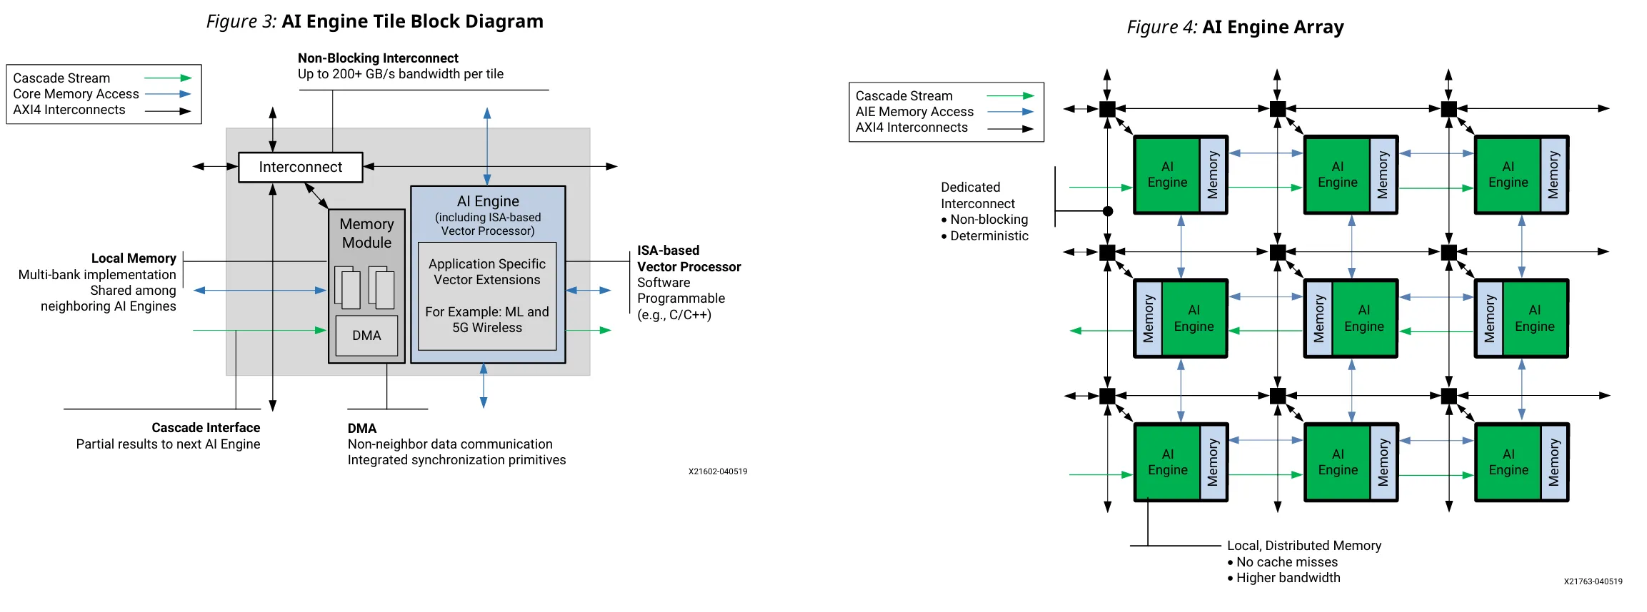
\includegraphics[width=1\linewidth]{archie.png}
    \caption{Cấu trúc chi tiết của AI Engine Tile}
\end{figure}

\begin{itemize}
    \item Tile interconnect: quản lý dữ liệu chạy vào tile qua NoC, PL và được định tuyến tới RAM

    \item AIE Core: có thể lập trình bằng C/C++,… tối ưu cho tính toán song song, có thể cấu hình cho ứng dụng cụ thể, truyền kết quả trung gian tới tile kế tiếp

    \item Memory Module:
    \begin{itemize}
        \item Bao gồm: \textbf{32KB RAM} chia thành 8 bank, DMA, cơ chế đồng bộ giữa các tile.
        \item Khả năng truy cập chéo: mỗi tile có thể truy cập:
        \begin{itemize}
            \item RAM của chính nó.
            \item RAM của tile phía Bắc (North).
            \item RAM của tile phía Nam (South).
            \item RAM của tile phía Đông hoặc Tây (East/West) tùy vào vị trí dòng.
        \end{itemize}
    \end{itemize}

    \item Cascade interface: Các tile được kết nối theo hướng zigzag và hướng lên trên (như minh họa ở Hình 4)
\end{itemize}

\section{Truy cập tài nguyên qua AXI4 MM}

Master AXI4 kết nối vào NoC có thể: đọc ghi RAM của tile, cấu hình bộ DMA, viết lệnh vào thanh ghi control, debug lỗi,…
\begin{figure}[H]
    \centering
    \includegraphics[width=0.75\linewidth]{Pictures/imagecode .png}
    \caption{Địa chỉ giao diện AXI4}
\end{figure}
Cấu trúc địa chỉ: \begin{itemize}
    \item column: tối đa 128 cột
    \item row: tối đa 32 hàng 
    \item tile: offset bên trong tile (để ghi vào thanh ghi, RAM, DMA,…)
\end{itemize}
Ví dụ: Viết từ CPU ARM: ghi 0x42 vào offset 0x100 của tile tại (row=3, col=10): 
\lstinputlisting[style=cstyle, caption={Code}]{codeex.tex}
\section{AXI4-Stream Interconnect\cite{amdAM009}.} 

 Mỗi AIE có 1 AXI4-stream interconnect giúp truyền dữ liệu giữa các tile, cấu hình tĩnh, thông qua giao diện bộ nhớ, có thể lập trình được.\\
 Chức năng: quản lý backpressure (điều tiết dữ liệu khi phía nhận bị nghẽn), đảm bảo băng thông tối đa.\\
 Cấu trúc thành phần:
\begin{itemize}
    \item Port Handlers:
    Điều khiển luồng vào/ra tại mỗi cổng.
    Chọn tuyến đường cho dữ liệu.
    \item FIFOs:
    Hai buffer (bộ đệm) 16 hàng, mỗi hàng rộng 32-bit + 1-bit TLAST.
    Có thể xâu chuỗi (chaining) để tạo độ trễ hoặc buffer dữ liệu.
    \item Arbiters (bộ chọn):
    Sáu bộ chọn lập trình được. 
    Dùng trong chế độ packet switching để phân xử khi nhiều luồng tranh tài nguyên.
    \item Stream Switch Configuration Registers:
    Các thanh ghi cấu hình dùng để thiết lập đường truyền (circuit hoặc packet-switched).
\end{itemize}
\begin{figure}[H]
    \centering
    \includegraphics[width=0.7\linewidth]{Pictures/fig6.png}
    
    \label{fig:enter-label}
\end{figure}
Khối trung tâm chứa các thành phần đã được liệt kê ở trên.\\
Lối vào: 
\begin{itemize}
    \item 4 hướng dữ liệu từ các phía
    \item Form AIE: dữ liệu được tile này sinh ra
    \item From DMA: dữ liệu từ bộ DMA, 
    \item From FIFO: dữ liệu từ bộ FIFO nội bộ
    \item Còn lại là dùng cho debug,...
\end{itemize}
Lối ra: 
\begin{itemize}
    \item 4 hướng dữ liệu đến các phía
    \item To AIE: dữ liệu được gửi đến tile này
    \item To DMA: dữ liệu chuyển tiếp đến nơi khác 
    \item To FIFO: lưu dữ liệu vào FIFO nội bộ
    \item To Register Configuration – cấu hình tuyến hoặc điều khiển chuyển mạch
\end{itemize}

\begin{figure}[H]
    \centering
    \includegraphics[width=0.8\linewidth]{Pictures/table2.png}

    \label{fig:enter-label}
\end{figure}
Ví dụ: nếu tile này muốn gửi dữ liệu sang tile phía đông: dữ liệu từ From AIE đến đầu ra East.

\section{AI Engine Tile Program Memory\cite{amdAM009}}
AIE có bộ nhớ 16KB để lưu câu lệnh VLIW. Có 2 giao diện để quản lý: 
\begin{itemize}
    \item Memory-mapped AXI4 interface: External master có thể đọc/ghi program memory thông qua Memory-mapped AXI4. 
    \item AIE interface:  AIE có giao diện rộng 128bit để nạp lệnh, chỉ có thể đọc mà không thể ghi đến program memory 
\end{itemize}
Để \textbf{truy cập đồng thời cả AIE và AXI4}: Bộ nhớ chia thành nhiều bank, mỗi bên truy cập không trùng nhau. Nếu truye cập trùng, cần có arbitration logic để tránh xung đột, ưu tiên luồng nào trước.

\section{AI Engine Interfaces}
Đọc thêm tại trang 17, tài liệu \cite{amdAM009}.
\begin{table}[h!]
\centering
\caption{Tóm tắt nhanh các giao diện của AI Engine}
\begin{tabular}{l l c}
\hline
\textbf{Giao diện} & \textbf{Mục đích chính} & \textbf{Băng thông / Độ rộng} \\
\hline
Data Memory & Đọc/ghi dữ liệu nội tile & 2×256b load, 1×256b store \\
\hline
Program Memory & Fetch lệnh từ bộ nhớ & 128b \\
\hline
AXI4-Stream (Direct) & Gửi/nhận dữ liệu qua các stream chuẩn & 4×32b (2 in, 2 out) \\
\hline
Cascade Stream & Truyền accumulator giữa tile liền kề & 384b \\
\hline
Debug & Truy cập thanh ghi, hỗ trợ debug & AXI4 \\
\hline
Lock Interface & Đồng bộ hóa hoạt động giữa các tile & -- \\
\hline
Stall Handling & Điều khiển tạm dừng do xung đột hoặc tranh chấp & -- \\
\hline
Event Interface & Giao diện sinh/tạo sự kiện & 16b \\
\hline
Tile Timer & Đếm thời gian nội bộ tile & 64b \\
\hline
\end{tabular}
\end{table}

\section{AIE Architechture}


AIE là bộ xử lý được tối ưu cho:
\begin{itemize}
    \item Single-instruction multiple-data: cho phép thực thi 1 lệnh trên nhiều dư liệu 1 lúc, giúp tăng tốc xử lý các vecto, ví dụ như nhiều phần tử trong ma trận cùng lúc.
    \item Very-long instruction word: cho phép đóng gói nhieeufleenhj vào 1 từ lệnh dài, giúp xử lý song song nhiều lệnh trên 1 chu kì.
    \item Hỗ trợ dấy phẩy động và dấu phẩy tĩnh.
\end{itemize}
Các chức năng của AIE: 
\begin{figure}[H]
    \centering
    \includegraphics[width=0.9\linewidth]{Pictures/fig21.png}
  
    \label{fig:enter-label}
\end{figure}
\begin{itemize}
    \item \textbf{Scalar unit}: Bộ xử lý RISC 32-bit dạng scalar
    \begin{itemize}
        \item Có thanh ghi chung để lưu trữ con trỏ và thanh ghi cấu hình
        \item Hỗ trợ các hàm toán học phi tuyến
        \item Scalar ALU: Bộ xử lý logic số học đơn lẻ, có thể thực hiện nhân 2 số 32 bit scalar
        \item Có khả năng chuyển đổi giữa số nguyên và phẩy động
    \end{itemize}
    \item \textbf{AGU}: 3 bộ sinh địa chỉ  để đọc/ghi dữ liệu từ/to bộ nhớ:
    \begin{itemize}
        \item 2 AGU để load, 1 AGU để lưu
    \end{itemize}
    \begin{itemize}
        \item hỗ trợ nhiều chế độ địa chỉ: địa chỉ không đổi, địa chỉ từ thanh ghi,...
        \item FFT Address Generation: Có phần cứng riêng để tạo địa chỉ đặc biệt phục vụ biến đổi Fourier nhanh (FFT).
    \end{itemize}
    \item  \textbf{Vector fixed-point/integer unit}:
    \begin{itemize}
        \item 32 phép nhân 16-bit có thể được thực hiện mỗi chu kỳ trên một AI Engine tile.
        \item Hỗ trợ phép nhân tích lũy (MAC – Multiply and Accumulate) song song trên nhiều “lane” (đường dữ liệu song song). 
        \item Hỗ trợ dữ liệu real và complex với nhiều độ rộng bit khác nhau (8, 16, 32). (Bảng dưới)
        
        \begin{figure}[H]
        \centering
        \includegraphics[width=0.8\linewidth]{Pictures/table6.png}
        
        \label{fig:enter-label}
    \end{figure}
        \item X, Z là 2 vector đầu vào, X từ thanh ghi 1024 bit và Z từ thanh ghi 256 bit. Do số lương phần tử của Z ít hơn, nên sẽ được sao chép (broadcast) đến nhiều lane để tận dụng tối đa X. Có 128 bộ nhân 8 bit, và kết qua được cộng, lưu vào accumulator.
    \end{itemize}
    \item SPFP (Single-Precision Floating-Point) Vector Unit: Hỗ trợ dấu phẩy động đơn 32bit. Có thể xử lý song song trên nhiều lane, thực hiện 8 đơn vị MAC trên 1 chu kỳ(?)
    \item  \textbf{3 cổng truy cập dữ liệu}: 2 đọc, 1 ghi, có thể hoạt động đồng thời, cần tối ưu layout để tránh xung đột bank, gây stall toàn bộ pipeline.
    \item \textbf{VLIW Function:} Hỗ trợ phát nhiều lệnh tới tất cả function unit, nhiều định dạng khác nhau, độ dài lệnh khác nhau. Tối đa 7 lệnh thực hiện song song trong 1 chu kì.
    
\end{itemize}


    





\newpage
\section{Code Bài tập nhân ma trận AI Engine}
\lstinputlisting[style=cstyle, caption={Code}]{code_mmul.c}
 tài liệu API chính thức của AMD \cite{UG1079}, \cite{MMUL_API}
bài viết giải thích từ Xilinx \cite{XUP_Explained}, và hướng dẫn phòng lab chi tiết \cite{XUP_Lab}.

